\section{Multitask pretraining}

\newsavebox{\multitaskbrainage}
\sbox{\multitaskbrainage}{
    \multitaskbox{0}
}
\newsavebox{\multitaskmultitask}
\sbox{\multitaskmultitask}{
    \multitaskbox{1}
}

\newcommand{\featureplot}[2]{
    \begin{tikzpicture}
        \begin{axis}[
            view={0}{90},
            colorbar,
            colormap/temp,
            mesh/cols=64,
            height=7cm,
            width=7cm,
            xmajorticks=false,
            ymajorticks=false,
            xlabel={Features},
            ylabel={Features},
            point meta min=#2,
            point meta max=1,
            xmin=-0.5,
            xmax=63.5,
            ymin=-0.5,
            ymax=63.5,
            colorbar style={
                tick style={draw=none}
            }
        ]
        \addplot [
            matrix plot,
            mesh/cols=64,
            point meta=explicit,
            draw=black,
            draw opacity=0.1
        ] table [col sep=comma, meta index=2] {#1};

        \end{axis}
    \end{tikzpicture}
}

\newsavebox{\featurecorrelations}
\sbox{\featurecorrelations}{
    \featureplot{data/feature_correlations.csv}{0}
}
\newsavebox{\multicorrelations}
\sbox{\multicorrelations}{
    \featureplot{data/sfcn-multi.csv}{-1}
}

\begin{frame}{Multitask pretraining}
    \begin{tikzpicture}
        \node[draw=black] at (-5.25, -3.75) {};
        \node[draw=black] at (5.25, 3.5) {};

        \def\xmin{-2.55}
        \def\ymin{1}
        \def\nodedepth{0.066}
        \def\nodesize{0.15}

        \visible<1>{
            \node[anchor=south, text depth=0] at (\xmin + 2.675, \ymin + 1.43) {
                \textbf{Convolutional neural network}
            };
            \draw[thick, dashed] (\xmin + 0.22, \ymin + 1.43) --
            (\xmin + 5.13, \ymin + 1.43) --
            (\xmin + 5.13, \ymin - 1.42) --
            (\xmin + 0.22, \ymin - 1.42) -- cycle;

            \convlayer{\xmin - 0.06 + 0.4}{\ymin + 2.5 * \nodesize}{\nodedepth}{\nodesize}{12}{3}{blue}

            \node[] (firstfeatures) at (-0.95, -2) {
                \usebox{\firstfeaturespace}
            };

            \cnnarrow{(\xmin + 0.95, \ymin)}{(\xmin+2.2, \ymin)}{blue}
            \convlayer{\xmin + 1.44 + 0.4}{\ymin + 1.5 * \nodesize}{\nodedepth}{\nodesize}{8}{5}{blue}

            \node[] (secondfeatures) at (0.38, -2) {
                \usebox{\secondfeaturespace}
            };

            \cnnarrow{(\xmin + 2.43, \ymin)}{(\xmin+3.5, \ymin)}{blue}
            \convlayer{\xmin + 2.77 + 0.4}{\ymin + 0.5 * \nodesize}{\nodedepth}{\nodesize}{4}{7}{blue}

            \node[] (thirdfeatures) at (1.56, -2) {
                \usebox{\thirdfeaturespace}
            };

            \cnnarrow{(\xmin + 3.75, \ymin)}{(\xmin+5, \ymin)}{blue}
            \convlayer{\xmin + 3.93 + 0.4}{\ymin + 0}{\nodedepth}{\nodesize}{2}{9}{blue}

        }
        \visible<2-3>{
            \node[inner sep=0pt, draw=black] at (0, 2) {
                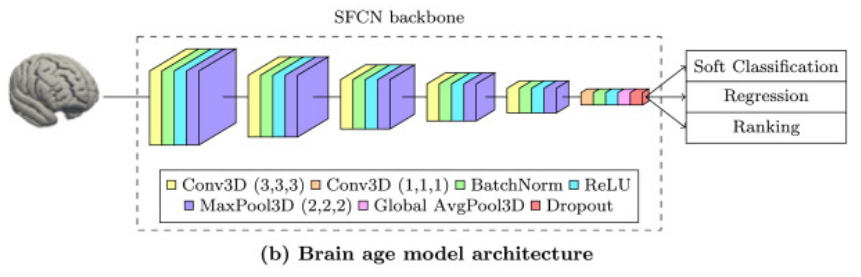
\includegraphics[width=8cm]{data/brainagemodel.png}
            };

            \node[anchor=south, text width=10.5cm, font=\tiny, align=flush center] at (0, -3.95) {
                Leonardsen, E. H., Peng, H., Kaufmann, T., Agartz, I., Andreassen, O. A., Celius, E. G., ... \& Wang, Y. (2022). "Deep neural networks learn general and clinically relevant representations of the ageing brain". \textit{NeuroImage, 256}, 119210.
            };
        }
        \visible<3>{
            \node[text width=10.5cm, align=flush center] at (0, -1.4) {
                \textit{"Furthermore, we see this result as evidence that deep learning models trained to predict age in large multisite datasets constitute excellent starting points for transfer learning, which can subsequently be fine-tuned to a variety of tasks."}\\
                - Esten et al.
            };
        }
        \visible<4>{
            \node[inner sep=0pt, draw=black] at (0, 0) {
                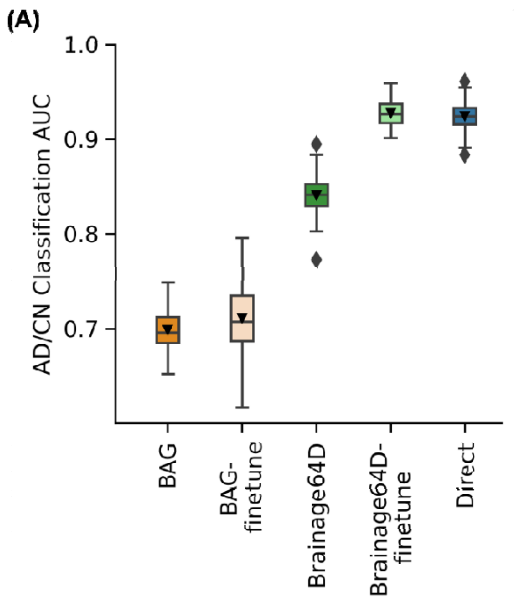
\includegraphics[width=4.5cm]{data/yeo.png}
            };
            \node[anchor=south, text width=10.5cm, font=\tiny, align=flush center] at (0, -3.95) {
                Tan, T. W. K., Nguyen, K. N., Zhang, C., Kong, R., Cheng, S. F., Ji, F., ... \& B. T. Thomas Yeo. (2024). "Evaluation of Brain Age as a Specific Marker of Brain Health". \textit{bioRxiv}, 2024-11.
            };
        }
        \visible<5>{
            \node[] at (0, 0) {
                \usebox{\multitaskbrainage}
            };
            \node[draw=red, thick, minimum height=1.2cm, minimum width=0.1cm] at (0.99, 0) {};
        }
        \visible<6>{
            \node[] at (0, 0) {
                \usebox{\featurecorrelations}
            };
        }
        \visible<7>{
            \node[] at (0, 0) {
                \usebox{\multitaskmultitask}
            };
        }
        \visible<8>{
            \node[] at (0, 0) {
                \usebox{\multicorrelations}
            };
        }
        \visible<9>{
            \node[] at (0, 0) {
                Brain age predictions
            };
        }
        \visible<10>{
            \node[] at (0, 0) {
                Brain age transfer learning
            };
        }
        \visible<11>{
            \node[] at (0, 0) {
                AD transfer learning
            };
        }
    \end{tikzpicture}
\end{frame}
